\part{Tercer semestre}
\chapterimage{3.pdf}
\chapter{Geometría y Trigonometría} %( 3 horas)


\section{Conceptos básicos}

\subsection{Bosquejo histórico de la Geometría}
La geometría, una de las ramas más antiguas de las matemáticas, ha evolucionado a lo largo de los siglos, desde sus orígenes en la antigüedad hasta las formas más avanzadas de geometría moderna. Los antiguos egipcios y babilonios ya empleaban principios geométricos para resolver problemas prácticos, como la medición de tierras y la construcción de estructuras. Euclides, en su obra \emph{Los Elementos}, sistematizó gran parte del conocimiento geométrico de su tiempo, estableciendo axiomas y teoremas fundamentales que aún se estudian hoy en día. La geometría ha crecido para incluir no solo la geometría euclidiana clásica, sino también otras formas como la geometría no euclidiana, que exploran espacios curvos y multidimensionales.

\subsection{Términos no definidos}
En la geometría, ciertos conceptos se consideran primitivos o indefinibles porque no se explican mediante otros conceptos más básicos. Estos incluyen:
\begin{itemize}
    \item \textbf{Punto}: Una entidad sin dimensiones, que indica una posición en el espacio.
    \item \textbf{Línea (o recta)}: Una serie infinita de puntos que se extiende en ambas direcciones sin fin y sin ancho.
    \item \textbf{Plano}: Una superficie bidimensional que se extiende infinitamente en todas las direcciones.
\end{itemize}

\subsection{Postulados de la Recta}
Los postulados de la recta son afirmaciones aceptadas sin demostración que sirven como base para la geometría euclidiana. Algunos de los postulados de la recta incluyen:
\begin{enumerate}
    \item A través de dos puntos distintos pasa una única línea recta.
    \item Un segmento de línea puede prolongarse indefinidamente en ambas direcciones.
    \item Una línea recta puede dividir un plano en dos regiones distintas.
\end{enumerate}

\subsection{Axiomas de la Geometría}
Los axiomas de la geometría son proposiciones que se aceptan como verdaderas sin pruebas y que sirven como base para la deducción de otros teoremas. Algunos de los axiomas fundamentales incluyen:
\begin{enumerate}
    \item Los objetos iguales a un mismo objeto son iguales entre sí.
    \item Si se añaden cantidades iguales a cantidades iguales, los totales son iguales.
    \item Si se restan cantidades iguales de cantidades iguales, los restos son iguales.
\end{enumerate}

\subsection{Terminología y notación}
La terminología y notación en geometría son esenciales para una comunicación clara y precisa. Algunas notaciones comunes incluyen:
\begin{itemize}
    \item \textbf{Puntos}: Generalmente representados por letras mayúsculas (A, B, C, etc.).
    \item \textbf{Líneas}: Denotadas por letras minúsculas (l, m, n) o por dos puntos (AB).
    \item \textbf{Ángulos}: Representados por el símbolo $\angle$ seguido de tres letras, donde la letra del medio representa el vértice (ej. $\angle ABC$).
    \item \textbf{Segmentos de línea}: Denotados por dos puntos con una línea encima (ej. $\overline{AB}$).
    \item \textbf{Planos}: Representados por letras griegas (ej. plano $\alpha$, plano $\beta$).
\end{itemize}


\section{Ángulos} %(6 horas)

\subsection{Definición, clasificación de los ángulos}
Un ángulo es la figura formada por dos rayos que comparten un extremo común, llamado vértice del ángulo. Los ángulos se pueden clasificar de varias maneras:
\begin{itemize}
    \item \textbf{Ángulo agudo}: mide menos de 90°.
    \item \textbf{Ángulo recto}: mide exactamente 90°.
    \item \textbf{Ángulo obtuso}: mide más de 90° pero menos de 180°.
    \item \textbf{Ángulo llano}: mide exactamente 180°.
    \item \textbf{Ángulo completo}: mide 360°.
\end{itemize}

\subsection{Teorema de los ángulos opuestos por el vértice}
El teorema de los ángulos opuestos por el vértice establece que, cuando dos líneas se cruzan, los ángulos opuestos por el vértice son congruentes. Esto significa que tienen la misma medida.

\subsection{Ángulos que se forman entre parejas de rectas cortadas por una transversal}
Cuando una recta transversal corta dos rectas, se forman varios tipos de ángulos, incluyendo:
\begin{itemize}
    \item \textbf{Ángulos correspondientes}: Ángulos que están en el mismo lado de la transversal y en la misma posición relativa con respecto a las dos rectas.
    \item \textbf{Ángulos alternos internos}: Ángulos que están en lados opuestos de la transversal pero dentro de las dos rectas.
    \item \textbf{Ángulos alternos externos}: Ángulos que están en lados opuestos de la transversal pero fuera de las dos rectas.
    \item \textbf{Ángulos colaterales internos (suplementarios)}: Ángulos que están en el mismo lado de la transversal y entre las dos rectas.
\end{itemize}

\subsection{Problemas relativos a ángulos}
En esta sección se resolverán problemas aplicando los conceptos y teoremas discutidos.

 

\subsection{Terminología y notación}
La terminología y notación en geometría son esenciales para una comunicación clara y precisa. Algunas notaciones comunes incluyen:
\begin{itemize}
    \item \textbf{Puntos}: Generalmente representados por letras mayúsculas (A, B, C, etc.).
    \item \textbf{Líneas}: Denotadas por letras minúsculas (l, m, n) o por dos puntos (AB).
    \item \textbf{Ángulos}: Representados por el símbolo $\angle$ seguido de tres letras, donde la letra del medio representa el vértice (ej. $\angle ABC$).
    \item \textbf{Segmentos de línea}: Denotados por dos puntos con una línea encima (ej. $\overline{AB}$).
    \item \textbf{Planos}: Representados por letras griegas (ej. plano $\alpha$, plano $\beta$).
\end{itemize}




\section{Paralelismo y Perpendicularidad} % (6 horas)

\subsection{Definición: característica del paralelismo y la perpendicularidad}

En geometría, el \textbf{paralelismo} y la \textbf{perpendicularidad} son conceptos fundamentales que describen la relación entre dos o más líneas.

\subsubsection{Paralelismo}

Dos líneas son \textbf{paralelas} si y solo si nunca se intersectan y mantienen una distancia constante entre sí en todos sus puntos. Matemáticamente, se dice que dos líneas \( l_1 \) y \( l_2 \) son paralelas si la pendiente de \( l_1 \) es igual a la pendiente de \( l_2 \), en el caso de que ambas líneas estén expresadas en forma pendiente-intersección.

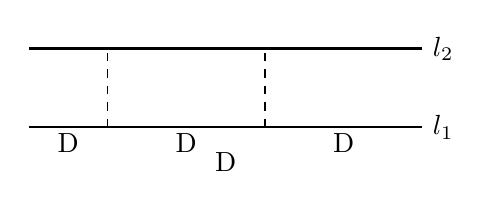
\begin{tikzpicture}
    \draw[thick] (0,0) -- (5,0) node[right] {$l_1$};
    \draw[thick] (0,1) -- (5,1) node[right] {$l_2$};
    \draw[dashed] (1,0) -- (1,1);
    \draw[dashed] (3,0) -- (3,1);
    \node at (0.5, -0.2) {D};
    \node at (2, -0.2) {D};
    \node at (4, -0.2) {D};
    \node[below] at (2.5, -0.2) {D};
\end{tikzpicture}

Donde \( D \) representa la distancia constante entre las dos líneas paralelas.

\subsubsection{Perpendicularidad}

Dos líneas son \textbf{perpendiculares} si se intersectan formando ángulos rectos, es decir, ángulos de \( 90^\circ \). Matemáticamente, si las pendientes de dos líneas \( m_1 \) y \( m_2 \) son tales que \( m_1 \cdot m_2 = -1 \), entonces las líneas son perpendiculares.

\begin{tikzpicture}
    \draw[thick] (0,0) -- (4,0) node[right] {$l_1$};
    \draw[thick] (2,-2) -- (2,2) node[above] {$l_2$};
    \draw[dashed] (2,0) -- (2,-1.5);
    \draw[dashed] (0,0) -- (2,-1.5);
    \draw[fill=black] (2,0) circle (2pt);
    \node at (2.3, 0.2) {90$^\circ$};
\end{tikzpicture}

Aquí, la intersección de las dos líneas forma un ángulo recto.

\subsection{Postulado del Paralelismo}

El \textbf{Postulado del Paralelismo} establece que dado un punto y una línea no contenida en el punto, existe una única línea que pasa por el punto y es paralela a la línea dada. Este postulado es uno de los axiomas fundamentales en la geometría euclidiana.

\subsection{Teorema Fundamental del Paralelismo}

Uno de los teoremas fundamentales del paralelismo es el \textbf{Teorema de la Alternancia de Ángulos}, que establece que si dos líneas paralelas son cortadas por una transversal, entonces los ángulos alternos internos son iguales.

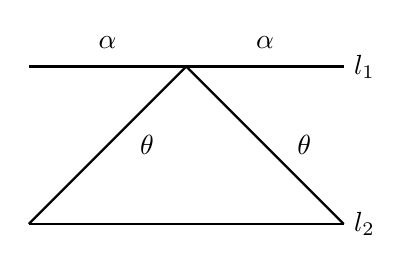
\begin{tikzpicture}
    \draw[thick] (0,0) -- (4,0) node[right] {$l_1$};
    \draw[thick] (0,-2) -- (4,-2) node[right] {$l_2$};
    \draw[thick] (0,-2) -- (2,0);
    \draw[thick] (2,0) -- (4,-2);
    \node at (1.5, -1) {$\theta$};
    \node at (3.5, -1) {$\theta$};
    \node at (1, 0.3) {$\alpha$};
    \node at (3, 0.3) {$\alpha$};
\end{tikzpicture}

En el gráfico, los ángulos alternos internos \(\alpha\) y \(\theta\) son iguales.

\subsection{Problemas de Demostración}
% TODO
% \textbf{Problema 1:} Demuestra que si dos líneas son perpendiculares a una misma línea, entonces son paralelas entre sí.

% \textbf{Solución:} Sea \( l_1 \) y \( l_2 \) dos líneas perpendiculares a una línea \( l \). Como \( l_1 \) y \( l_2 \) son perpendiculares a \( l \), ambas forman ángulos rectos con \( l \). Así, los ángulos entre \( l_1 \) y \( l \) y entre \( l_2 \) y \( l \) son iguales, lo que implica que los ángulos entre \( l_1 \) y \( l_2 \) también son iguales. Por lo tanto, \( l_1 \) y \( l_2 \) son paralelas.

% \textbf{Problema 2:} Demuestra que la suma de los ángulos internos de un triángulo es igual a \( 180^\circ \) utilizando el concepto de paralelismo.

% \textbf{Solución:} Dibuja una línea paralela a uno de los lados del triángulo a través del vértice opuesto. Luego, usa el postulado del paralelismo para mostrar que los ángulos internos del triángulo se corresponden con los ángulos alternos internos y ángulos internos de la línea paralela. La suma de estos ángulos será \( 180^\circ \) debido a que forman una línea recta.


\section{Triángulos} % (4.5 horas)

El estudio de los triángulos es fundamental en geometría, ya que proporciona una base sólida para entender muchas propiedades geométricas. Esta sección se enfoca en la definición, clasificación y propiedades de los triángulos, así como en las rectas y puntos notables.

\subsection{Definición y Clasificación de los Triángulos}

Un \textbf{triángulo} es una figura geométrica formada por tres segmentos de línea que se encuentran en tres puntos no colineales, llamados \textbf{vértices}. Los segmentos de línea son los \textbf{lados} del triángulo.

\subsubsection{Clasificación según los Ángulos}

Los triángulos se clasifican en función de sus ángulos internos:

\begin{itemize}
    \item \textbf{Triángulo Acutángulo:} Todos sus ángulos son menores a \( 90^\circ \).
    \item \textbf{Triángulo Rectángulo:} Tiene un ángulo de \( 90^\circ \).
    \item \textbf{Triángulo Obtusángulo:} Tiene un ángulo mayor a \( 90^\circ \).
\end{itemize}

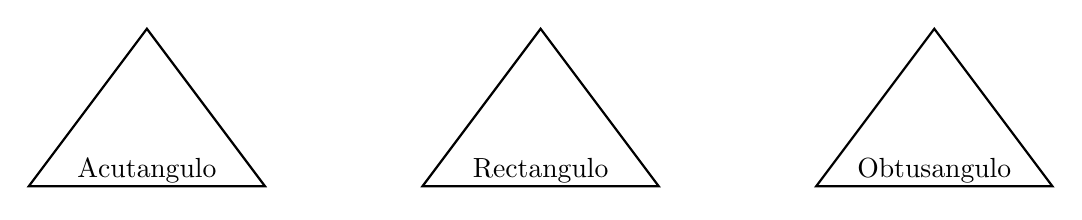
\begin{tikzpicture}
    \draw[thick] (0,0) -- (3,0) -- (1.5,2) -- cycle;
    \node at (1.5, 0.2) {Acutangulo};
    \draw[thick] (5,0) -- (8,0) -- (6.5,2) -- cycle;
    \node at (6.5, 0.2) {Rectangulo};
    \draw[thick] (10,0) -- (13,0) -- (11.5,2) -- cycle;
    \node at (11.5, 0.2) {Obtusangulo};
\end{tikzpicture}

\subsubsection{Clasificación según los Lados}

Los triángulos también se clasifican según la longitud de sus lados:

\begin{itemize}
    \item \textbf{Triángulo Equilátero:} Todos sus lados son de igual longitud.
    \item \textbf{Triángulo Isósceles:} Tiene dos lados de igual longitud.
    \item \textbf{Triángulo Escaleno:} Todos sus lados son de diferente longitud.
\end{itemize}

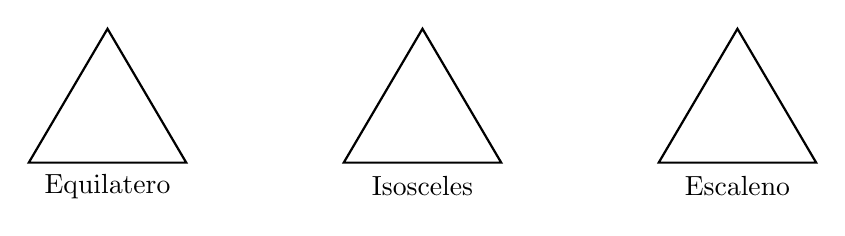
\begin{tikzpicture}
    \draw[thick] (0,0) -- (2,0) -- (1,1.7) -- cycle;
    \node at (1, -0.3) {Equilatero};
    \draw[thick] (4,0) -- (6,0) -- (5,1.7) -- cycle;
    \node at (5, -0.3) {Isosceles};
    \draw[thick] (8,0) -- (10,0) -- (9,1.7) -- cycle;
    \node at (9, -0.3) {Escaleno};
\end{tikzpicture}

\subsection{Teorema de los Ángulos Interiores de un Triángulo}

El \textbf{Teorema de los Ángulos Interiores} establece que la suma de los ángulos internos de un triángulo es siempre igual a \( 180^\circ \).

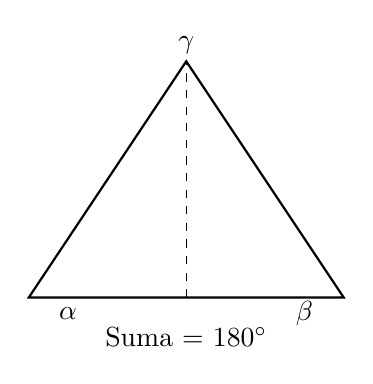
\begin{tikzpicture}
    \draw[thick] (0,0) -- (4,0) -- (2,3) -- cycle;
    \node at (0.5, -0.2) {$\alpha$};
    \node at (3.5, -0.2) {$\beta$};
    \node at (2, 3.2) {$\gamma$};
    \draw[dashed] (2,0) -- (2,3);
    \draw[dashed] (0,0) -- (2,3);
    \draw[dashed] (4,0) -- (2,3);
    \node at (2, -0.5) {Suma = 180$^\circ$};
\end{tikzpicture}

\subsection{Rectas y Puntos Notables de los Triángulos}

Los triángulos tienen varios puntos y rectas notables que son importantes para resolver problemas geométricos.

\subsubsection{Puntos Notables}

\begin{itemize}
    \item \textbf{Baricentro:} Punto de concurrencia de las medianas del triángulo.
    \item \textbf{Ortocentro:} Punto de concurrencia de las alturas del triángulo.
    \item \textbf{Circuncentro:} Punto de concurrencia de las mediatrices de los lados del triángulo.
    \item \textbf{Incentro:} Punto de concurrencia de las bisectrices de los ángulos del triángulo.
\end{itemize}

\subsubsection{Rectas Notables}

\begin{itemize}
    \item \textbf{Mediana:} Segmento que une un vértice con el punto medio del lado opuesto.
    \item \textbf{Altura:} Segmento perpendicular desde un vértice al lado opuesto.
    \item \textbf{Mediatriz:} Recta perpendicular a un lado del triángulo que pasa por su punto medio.
    \item \textbf{Bisectriz:} Recta que divide un ángulo en dos ángulos iguales.
\end{itemize}

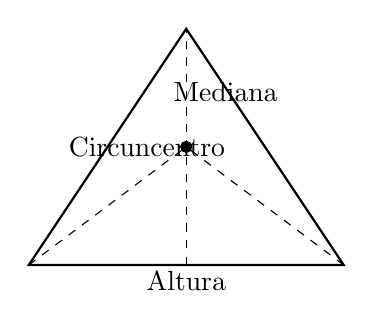
\begin{tikzpicture}
    \draw[thick] (0,0) -- (4,0) -- (2,3) -- cycle;
    \draw[dashed] (2,0) -- (2,3); % Altura
    \draw[dashed] (0,0) -- (2,1.5); % Mediana
    \draw[dashed] (4,0) -- (2,1.5); % Mediana
    \draw[fill=black] (2,1.5) circle (2pt); % Circuncentro
    \node at (2, -0.2) {Altura};
    \node at (2.5, 2.2) {Mediana};
    \node at (1.5, 1.5) {Circuncentro};
\end{tikzpicture}


\section{Congruencia} % (6 horas)

\subsection{Concepto de Congruencia}

Dos figuras geométricas son \textbf{congruentes} si tienen la misma forma y tamaño. Esto significa que se pueden superponer una sobre otra mediante una secuencia de transformaciones geométricas: traslaciones, rotaciones y reflexiones. En particular, dos triángulos son congruentes si sus ángulos y lados correspondientes son iguales.

\begin{center}
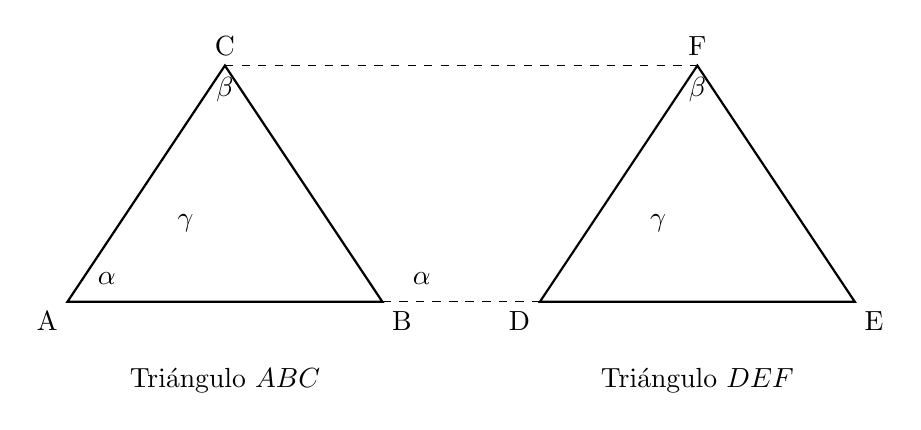
\begin{tikzpicture}
    % Triángulo 1
    \draw[thick] (0,0) -- (4,0) -- (2,3) -- cycle;
    \node at (0,0) [below left] {A};
    \node at (4,0) [below right] {B};
    \node at (2,3) [above] {C};
    
    % Triángulo 2
    \draw[thick] (6,0) -- (10,0) -- (8,3) -- cycle;
    \node at (6,0) [below left] {D};
    \node at (10,0) [below right] {E};
    \node at (8,3) [above] {F};
    
    \node at (2, -1) {Triángulo $ABC$};
    \node at (8, -1) {Triángulo $DEF$};
    
    % Líneas de congruencia
    \draw[dashed] (0,0) -- (6,0);
    \draw[dashed] (4,0) -- (10,0);
    \draw[dashed] (2,3) -- (8,3);
    
    % Etiquetas de ángulos
    \node at (0.5, 0.3) {$\alpha$};
    \node at (4.5, 0.3) {$\alpha$};
    \node at (2, 2.7) {$\beta$};
    \node at (8, 2.7) {$\beta$};
    \node at (1.5, 1) {$\gamma$};
    \node at (7.5, 1) {$\gamma$};
\end{tikzpicture}
\end{center}

En la figura anterior, los triángulos $ABC$ y $DEF$ son congruentes porque sus ángulos y lados correspondientes son iguales.

\subsection{Postulados de Congruencia}

Para determinar si dos triángulos son congruentes, se utilizan los siguientes postulados:

\begin{itemize}
    \item \textbf{Postulado Lado-Lado-Lado (LLL):} Si en dos triángulos, los tres lados de uno son iguales a los tres lados del otro, entonces los triángulos son congruentes.
    \item \textbf{Postulado Ángulo-Lado-Ángulo (ALA):} Si en dos triángulos, un ángulo y los dos lados adyacentes a ese ángulo son iguales a los correspondientes en otro triángulo, entonces los triángulos son congruentes.
    \item \textbf{Postulado Ángulo-Ángulo-Lado (AAL):} Si en dos triángulos, dos ángulos y el lado no comprendido entre ellos son iguales a los correspondientes en otro triángulo, entonces los triángulos son congruentes.
\end{itemize}

\subsection{Teorema del Triángulo Isósceles}

Un triángulo es \textbf{isósceles} si tiene al menos dos lados iguales. El teorema del triángulo isósceles establece que:

\begin{itemize}
    \item Los ángulos opuestos a los lados iguales son también iguales.
    \item La altura, mediana y bisectriz desde el vértice del ángulo de los dos lados iguales son coincidentes.
\end{itemize}

\begin{center}
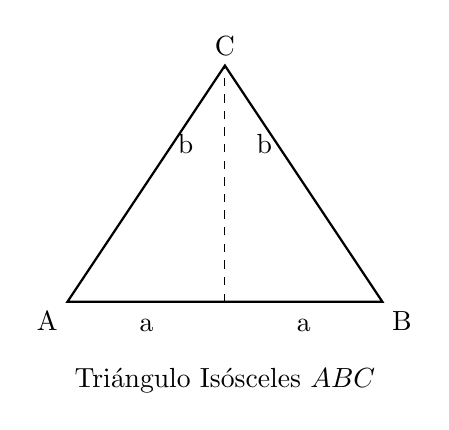
\begin{tikzpicture}
    % Triángulo Isósceles
    \draw[thick] (0,0) -- (4,0) -- (2,3) -- cycle;
    \node at (0,0) [below left] {A};
    \node at (4,0) [below right] {B};
    \node at (2,3) [above] {C};
    \draw[dashed] (2,0) -- (2,3);
    
    % Ángulos
    \node at (1, -0.3) {a};
    \node at (3, -0.3) {a};
    \node at (2.5, 2) {b};
    \node at (1.5, 2) {b};
    
    % Líneas
    \draw[dashed] (0,0) -- (2,3);
    \draw[dashed] (4,0) -- (2,3);
    \node at (2, -1) {Triángulo Isósceles $ABC$};
\end{tikzpicture}
\end{center}

\subsection{Problemas de Aplicación}

% \begin{enumerate}
%     \item Dado un triángulo con lados $AB = AC$ y ángulos $\angle ABC = \angle ACB$, demuestra que el triángulo es isósceles.
%     \item Usando los postulados de congruencia, demuestra que los triángulos formados al cortar un triángulo rectángulo por su mediana son congruentes.
%     \item Resuelve el siguiente problema: En un triángulo $XYZ$, si $XY = YZ$ y $\angle X = \angle Z$, ¿cómo se puede demostrar que el triángulo es isósceles?
% \end{enumerate}










\section{Semejanza} %(10.5 horas)

\subsection{Razones y Proporciones}

\begin{definition}
    \textbf{Razón:} Una razón es la relación entre dos magnitudes de la misma especie, expresada como una fracción o un cociente. 
\end{definition}

\begin{definition}
    \textbf{Proporción:} Una proporción es una igualdad entre dos razones. Se expresa como \(\frac{a}{b} = \frac{c}{d}\), donde \(a\), \(b\), \(c\) y \(d\) son magnitudes positivas.
\end{definition}

\begin{example}
    Consideremos las razones \(\frac{2}{3}\) y \(\frac{4}{6}\). Como \(\frac{2}{3} = \frac{4}{6}\), decimos que estas razones son proporcionales.
\end{example}

\subsection{Concepto de Semejanza. Triángulos Semejantes}

\begin{definition}
    \textbf{Semejanza de Triángulos:} Dos triángulos son semejantes si tienen sus ángulos correspondientes iguales y sus lados correspondientes proporcionales.
\end{definition}

\begin{example}
    Dos triángulos con ángulos iguales y lados proporcionales se llaman triángulos semejantes. Por ejemplo, si \(\triangle ABC \sim \triangle DEF\), entonces \(\frac{AB}{DE} = \frac{BC}{EF} = \frac{CA}{FD}\).
\end{example}

\subsection{Postulado de Semejanza}

\begin{definition}
    Los postulados de semejanza para triángulos son:
    \begin{itemize}
        \item \textbf{Postulado AAA:} Si dos triángulos tienen sus ángulos correspondientes iguales, entonces son semejantes.
        \item \textbf{Postulado LAL:} Si un ángulo y los dos lados adyacentes de un triángulo son proporcionales a un ángulo y los dos lados adyacentes de otro triángulo, entonces los triángulos son semejantes.
        \item \textbf{Postulado LLL:} Si los tres lados de un triángulo son proporcionales a los tres lados de otro triángulo, entonces los triángulos son semejantes.
    \end{itemize}
\end{definition}

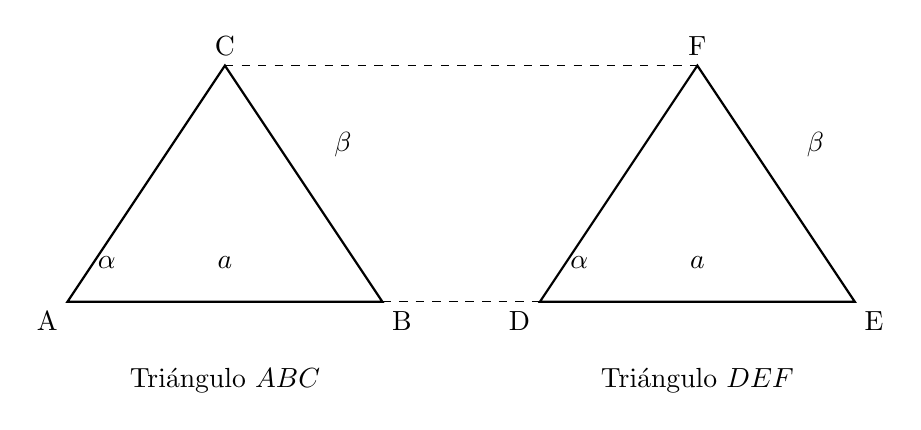
\begin{tikzpicture}
    % Triángulo AAA
    \draw[thick] (0,0) -- (4,0) -- (2,3) -- cycle;
    \node at (0,0) [below left] {A};
    \node at (4,0) [below right] {B};
    \node at (2,3) [above] {C};
    \node at (2, -1) {Triángulo $ABC$};
    
    % Triángulo similar AAA
    \draw[thick] (6,0) -- (10,0) -- (8,3) -- cycle;
    \node at (6,0) [below left] {D};
    \node at (10,0) [below right] {E};
    \node at (8,3) [above] {F};
    \node at (8, -1) {Triángulo $DEF$};
    
    % Líneas de semejanza
    \draw[dashed] (0,0) -- (6,0);
    \draw[dashed] (4,0) -- (10,0);
    \draw[dashed] (2,3) -- (8,3);
    
    % Etiquetas de ángulos
    \node at (0.5, 0.5) {$\alpha$};
    \node at (6.5, 0.5) {$\alpha$};
    \node at (3.5, 2) {$\beta$};
    \node at (9.5, 2) {$\beta$};
    \node at (2, 0.5) {$a$};
    \node at (8, 0.5) {$a$};
\end{tikzpicture}

\subsection{Teorema de Pitágoras}

\begin{theorem}[Teorema de Pitágoras]
    En un triángulo rectángulo, el cuadrado de la hipotenusa es igual a la suma de los cuadrados de los catetos. Es decir, si \(a\) y \(b\) son los catetos y \(c\) es la hipotenusa, entonces \(c^2 = a^2 + b^2\).
\end{theorem}

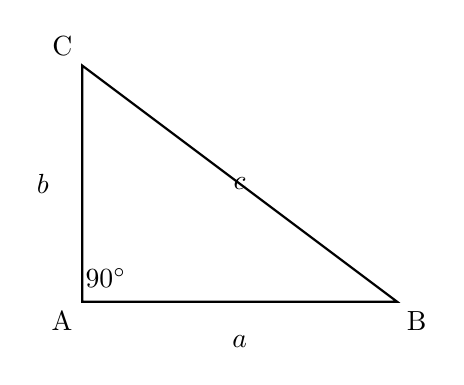
\begin{tikzpicture}
    % Triángulo Rectángulo
    \draw[thick] (0,0) -- (4,0) -- (0,3) -- cycle;
    \node at (0,0) [below left] {A};
    \node at (4,0) [below right] {B};
    \node at (0,3) [above left] {C};
    
    % Etiquetas de lados
    \node at (2, -0.5) {$a$};
    \node at (-0.5, 1.5) {$b$};
    \node at (2, 1.5) {$c$};
    
    % Ángulo recto
    \node at (0.3, 0.3) {$90^\circ$};
\end{tikzpicture}

\subsection{Teorema Fundamental de Proporcionalidad}

\begin{theorem}[Teorema Fundamental de Proporcionalidad]
    Si se traza una recta paralela a uno de los lados de un triángulo, entonces se forma un triángulo semejante al triángulo dado, y los segmentos de los otros dos lados son proporcionales.
\end{theorem}

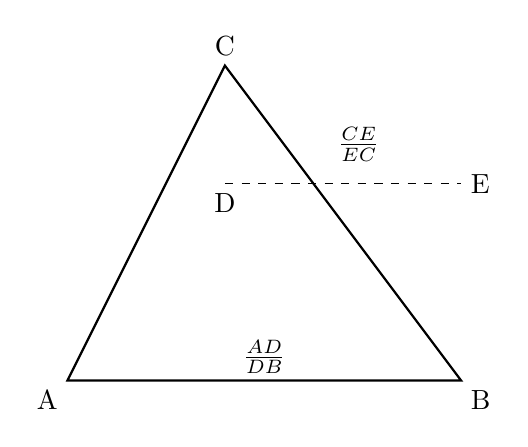
\begin{tikzpicture}
    % Triángulo y recta paralela
    \draw[thick] (0,0) -- (5,0) -- (2,4) -- cycle;
    \draw[dashed] (2,4) -- (5,0);
    \draw[dashed] (2,4) -- (0,0);
    \draw[dashed] (2,2.5) -- (5,2.5);
    
    % Etiquetas
    \node at (0,0) [below left] {A};
    \node at (5,0) [below right] {B};
    \node at (2,4) [above] {C};
    \node at (2,2.5) [below] {D};
    \node at (5,2.5) [right] {E};
    
    % Etiquetas de proporciones
    \node at (2.5, 0.3) {$\frac{AD}{DB}$};
    \node at (3.7, 3) {$\frac{CE}{EC}$};
\end{tikzpicture}


\section{Funciones Trigonométricas} %(7.5 horas)

\subsection{Introducción a la Trigonometría}

\begin{definition}
    \textbf{Trigonometría:} La trigonometría es la rama de las matemáticas que estudia las relaciones entre los ángulos y los lados de los triángulos. Su desarrollo histórico se remonta a las civilizaciones antiguas como los egipcios y babilonios, y fue formalmente desarrollada por los griegos y los indios en la antigüedad.
\end{definition}

\begin{itemize}
    \item \textbf{Breve semblanza histórica:} La trigonometría tiene sus raíces en la astronomía y la geometría. Los antiguos griegos, como Hiparco y Ptolomeo, hicieron contribuciones significativas, y la trigonometría se desarrolló aún más en la India y el mundo islámico durante la Edad Media.
    \item \textbf{Importancia para el Ingeniero Agrónomo:} La trigonometría es crucial para medir distancias inaccesibles y resolver problemas relacionados con la topografía y la geometría del terreno.
    \item \textbf{Objetivo general del curso:} Proporcionar una comprensión sólida de las funciones trigonométricas y su aplicación en la resolución de triángulos rectángulos.
    \item \textbf{Ubicación en el plan de estudios:} La trigonometría se ubica en el estudio de las matemáticas aplicadas, y es fundamental para la ingeniería y las ciencias aplicadas.
\end{itemize}

\subsection{Funciones Trigonométricas de un Ángulo Agudo de un Triángulo Rectángulo}

\begin{definition}
    \textbf{Funciones Trigonométricas:} Para un ángulo agudo en un triángulo rectángulo, las funciones trigonométricas principales son:
    \begin{itemize}
        \item \textbf{Seno} (\(\sin\)): \(\sin(\theta) = \frac{\text{lado opuesto}}{\text{hipotenusa}}\)
        \item \textbf{Coseno} (\(\cos\)): \(\cos(\theta) = \frac{\text{lado adyacente}}{\text{hipotenusa}}\)
        \item \textbf{Tangente} (\(\tan\)): \(\tan(\theta) = \frac{\text{lado opuesto}}{\text{lado adyacente}}\)
    \end{itemize}
\end{definition}

\begin{example}
    En un triángulo rectángulo con un ángulo de \(30^\circ\), si la hipotenusa es 10 unidades, entonces:
    \[
    \sin(30^\circ) = \frac{1}{2} \quad \text{y} \quad \text{lado opuesto} = 10 \times \frac{1}{2} = 5
    \]
\end{example}

\subsection{Manejo de Tablas y/o Calculadora}

\begin{definition}
    \textbf{Tablas y Calculadora:} Las tablas trigonométricas y las calculadoras permiten encontrar los valores de las funciones trigonométricas para ángulos dados. Es fundamental familiarizarse con su uso para resolver problemas de trigonometría de manera eficiente.
\end{definition}

\begin{example}
    Para encontrar \(\sin(45^\circ)\) usando una calculadora:
    \[
    \sin(45^\circ) \approx 0.707
    \]
\end{example}

\subsection{Triángulos Especiales}

\begin{definition}
    \textbf{Triángulos Especiales:} Existen triángulos rectángulos especiales que tienen ángulos de \(30^\circ\), \(45^\circ\) y \(60^\circ\). Estos triángulos tienen propiedades y razones trigonométricas específicas:
    \begin{itemize}
        \item Triángulo \(30^\circ-60^\circ-90^\circ\): Las longitudes de los lados están en la proporción 1 : \(\sqrt{3}\) : 2.
        \item Triángulo \(45^\circ-45^\circ-90^\circ\): Las longitudes de los lados están en la proporción 1 : 1 : \(\sqrt{2}\).
    \end{itemize}
\end{definition}

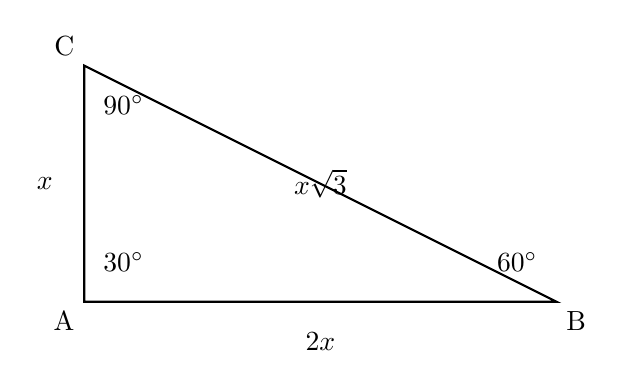
\begin{tikzpicture}
    % Triángulo 30-60-90
    \draw[thick] (0,0) -- (6,0) -- (0,3) -- cycle;
    \node at (0,0) [below left] {A};
    \node at (6,0) [below right] {B};
    \node at (0,3) [above left] {C};
    
    % Etiquetas
    \node at (3, -0.5) {$2x$};
    \node at (-0.5, 1.5) {$x$};
    \node at (3, 1.5) {$x\sqrt{3}$};
    
    % Ángulos
    \node at (0.5, 0.5) {$30^\circ$};
    \node at (5.5, 0.5) {$60^\circ$};
    \node at (0.5, 2.5) {$90^\circ$};
\end{tikzpicture}

\subsection{Solución de Triángulos Rectángulos, Cálculo de Áreas}

\begin{definition}
    \textbf{Solución de Triángulos Rectángulos:} Consiste en encontrar las longitudes de los lados y los ángulos de un triángulo rectángulo utilizando funciones trigonométricas. El área de un triángulo rectángulo se calcula como:
    \[
    \text{Área} = \frac{1}{2} \times \text{base} \times \text{altura}
    \]
\end{definition}

\begin{example}
    En un triángulo rectángulo con base 6 y altura 8, el área es:
    \[
    \text{Área} = \frac{1}{2} \times 6 \times 8 = 24
    \]
\end{example}

\subsection{Ángulos de Elevación y Depresión}

\begin{definition}
    \textbf{Ángulos de Elevación y Depresión:} El ángulo de elevación es el ángulo formado por la línea de visión hacia arriba desde un punto de observación. El ángulo de depresión es el ángulo formado por la línea de visión hacia abajo desde un punto de observación. Ambos se utilizan para resolver problemas de altura y distancia.
\end{definition}

\begin{tikzpicture}
    % Ángulo de elevación y depresión
    \draw[thick] (0,0) -- (5,0) -- (5,4) -- cycle;
    \draw[dashed] (0,0) -- (5,4);
    \draw[dashed] (5,0) -- (5,2);
    
    % Etiquetas
    \node at (0,0) [below left] {A};
    \node at (5,0) [below right] {B};
    \node at (5,4) [above right] {C};
    \node at (5,2) [right] {D};
    
    % Ángulos
    \node at (2.5, -0.5) {$\text{Distancia}$};
    \node at (5.5, 2) {$\text{Ángulo de Elevación}$};
    \node at (2.5, 4.5) {$\text{Ángulo de Depresión}$};
\end{tikzpicture}


\section{Funciones Trigonométricas} %(7.5 horas)

\subsection{Sistema de Coordenadas Rectangulares}

\begin{definition}
    \textbf{Sistema de Coordenadas Rectangulares:} El sistema de coordenadas rectangulares, también conocido como sistema de coordenadas cartesianas, está formado por dos ejes perpendiculares: el eje \(x\) (horizontal) y el eje \(y\) (vertical). Cada punto en el plano se localiza mediante un par de coordenadas \((x, y)\), donde \(x\) es la distancia desde el eje \(y\) y \(y\) es la distancia desde el eje \(x\).
\end{definition}

\subsection{Definir Grados y Radianes, Conversiones de un Sistema al Otro}

\begin{definition}
    \textbf{Grados y Radianes:} 
    \begin{itemize}
        \item \textbf{Grados:} Un círculo completo tiene 360 grados.
        \item \textbf{Radianes:} Un círculo completo tiene \(2\pi\) radianes. La conversión entre grados y radianes se realiza mediante las siguientes fórmulas:
        \[
        \text{Radianes} = \text{Grados} \times \frac{\pi}{180}
        \]
        \[
        \text{Grados} = \text{Radianes} \times \frac{180}{\pi}
        \]
    \end{itemize}
\end{definition}

\begin{example}
    Convertir \(45^\circ\) a radianes:
    \[
    45^\circ \times \frac{\pi}{180} = \frac{\pi}{4}
    \]
\end{example}

\subsection{Ángulo en Posición Normal, Concepto de Ángulo Reducido o de Referencia}

\begin{definition}
    \textbf{Ángulo en Posición Normal:} Un ángulo está en posición normal cuando su vértice está en el origen y uno de sus lados está en el eje positivo \(x\). Los ángulos se miden en sentido antihorario desde el eje positivo \(x\).
    
    \textbf{Ángulo Reducido o de Referencia:} Es el ángulo agudo formado entre el lado terminal del ángulo en posición normal y el eje \(x\).
\end{definition}

\begin{example}
    Para un ángulo de \(135^\circ\), el ángulo de referencia es \(180^\circ - 135^\circ = 45^\circ\).
\end{example}

\subsection{Definición de las Funciones Trigonométricas de un Ángulo Cualquiera en Posición Normal}

\begin{definition}
    \textbf{Funciones Trigonométricas en Posición Normal:} 
    \begin{itemize}
        \item \textbf{Seno} (\(\sin\)): La razón del lado opuesto al ángulo dividido por la hipotenusa.
        \item \textbf{Coseno} (\(\cos\)): La razón del lado adyacente al ángulo dividido por la hipotenusa.
        \item \textbf{Tangente} (\(\tan\)): La razón del seno sobre el coseno.
    \end{itemize}
\end{definition}

\begin{example}
    Para un ángulo de \(150^\circ\) (en el segundo cuadrante), el seno es positivo y el coseno es negativo. El ángulo de referencia es \(30^\circ\):
    \[
    \sin(150^\circ) = \sin(30^\circ) = \frac{1}{2}
    \]
    \[
    \cos(150^\circ) = -\cos(30^\circ) = -\frac{\sqrt{3}}{2}
    \]
\end{example}

\subsection{Signo de las Funciones Trigonométricas en los Cuatro Cuadrantes}

\begin{definition}
    \textbf{Signo de las Funciones Trigonométricas:} 
    \begin{itemize}
        \item \textbf{Primer Cuadrante} (\(0^\circ\) a \(90^\circ\)): \(\sin\), \(\cos\), y \(\tan\) son positivos.
        \item \textbf{Segundo Cuadrante} (\(90^\circ\) a \(180^\circ\)): \(\sin\) es positivo, \(\cos\) y \(\tan\) son negativos.
        \item \textbf{Tercer Cuadrante} (\(180^\circ\) a \(270^\circ\)): \(\tan\) es positivo, \(\sin\) y \(\cos\) son negativos.
        \item \textbf{Cuarto Cuadrante} (\(270^\circ\) a \(360^\circ\)): \(\cos\) es positivo, \(\sin\) y \(\tan\) son negativos.
    \end{itemize}
\end{definition}

\subsection{Ángulos Positivos, Ángulos Negativos}

\begin{definition}
    \textbf{Ángulos Positivos y Negativos:} 
    \begin{itemize}
        \item \textbf{Ángulos Positivos:} Se miden en sentido antihorario desde el eje \(x\).
        \item \textbf{Ángulos Negativos:} Se miden en sentido horario desde el eje \(x\).
    \end{itemize}
\end{definition}

\begin{example}
    Un ángulo de \(-30^\circ\) es equivalente a \(360^\circ - 30^\circ = 330^\circ\).
\end{example}

\subsection{Funciones Trigonométricas Inversas}

\begin{definition}
    \textbf{Funciones Trigonométricas Inversas:} Las funciones trigonométricas inversas son:
    \begin{itemize}
        \item \textbf{Arco seno} (\(\sin^{-1}\)): Determina el ángulo cuyo seno es el valor dado.
        \item \textbf{Arco coseno} (\(\cos^{-1}\)): Determina el ángulo cuyo coseno es el valor dado.
        \item \textbf{Arco tangente} (\(\tan^{-1}\)): Determina el ángulo cuyo tangente es el valor dado.
    \end{itemize}
\end{definition}

\begin{example}
    Para encontrar el ángulo cuyo seno es \(\frac{1}{2}\):
    \[
    \sin^{-1}\left(\frac{1}{2}\right) = 30^\circ
    \]
\end{example}


\section{Círculo Trigonométrico, Graficación de las Funciones Trigonométricas} %(4.5 horas)

\subsection{El Círculo Trigonométrico}

\begin{definition}
    \textbf{Círculo Trigonométrico:} Es un círculo con radio 1 centrado en el origen del sistema de coordenadas cartesianas. Los puntos en el círculo corresponden a los valores de las funciones trigonométricas de un ángulo.
\end{definition}

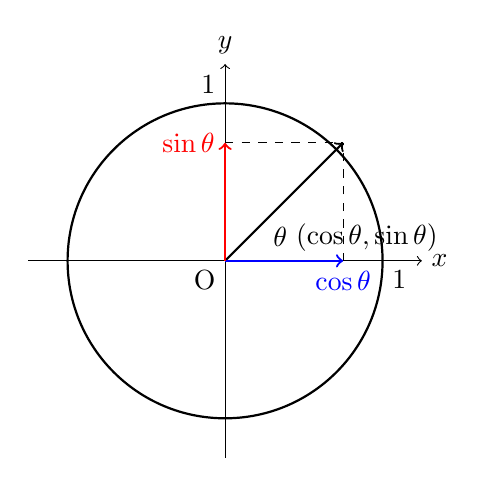
\begin{tikzpicture}
    % Draw the axes
    \draw[->] (-2.5,0) -- (2.5,0) node[right] {$x$};
    \draw[->] (0,-2.5) -- (0,2.5) node[above] {$y$};
    
    % Draw the unit circle
    \draw[thick] (0,0) circle(2);
    
    % Draw the angle
    \draw[thick, ->] (0,0) -- (1.5,1.5) coordinate (A) node[midway, above right]{};
    
    % Draw the radius line to the circle
    \draw[dashed] (0,0) -- (2,0) node[below right] {1};
    \draw[dashed] (0,0) -- (0,2) node[above left] {1};
    
    % Draw the cosine line
    \draw[thick, blue, ->] (0,0) -- (1.5,0) node[below] {$\cos\theta$};
    
    % Draw the sine line
    \draw[thick, red, ->] (0,0) -- (0,1.5) node[left] {$\sin\theta$};
    
    % Draw the tangent line
    % \draw[thick, green, ->] (1.5,0) -- (1.5,1.5) node[right] {$\tan\theta$};
    
    % Label the angle
    \node at (1.8, 0.3) {$(\cos\theta, \sin\theta)$};
    
    % Draw dashed lines
    \draw[dashed] (1.5,0) -- (1.5,1.5);
    \draw[dashed] (0,1.5) -- (1.5,1.5);
    
    % Draw the origin label
    \node at (0,0) [below left] {O};
    
    % Draw the angle label
    \node at (0.7, 0.3) {$\theta$};
\end{tikzpicture}

\subsection{Funciones Trigonométricas Definidas como Segmentos Rectilíneos}

\begin{definition}
    \textbf{Funciones Trigonométricas como Segmentos Rectilíneos:} Las funciones trigonométricas pueden ser representadas como segmentos rectilíneos en el círculo trigonométrico:
    \begin{itemize}
        \item \textbf{Seno} (\(\sin\theta\)): La coordenada \(y\) del punto en el círculo.
        \item \textbf{Coseno} (\(\cos\theta\)): La coordenada \(x\) del punto en el círculo.
        \item \textbf{Tangente} (\(\tan\theta\)): La razón de \(\sin\theta\) sobre \(\cos\theta\).
    \end{itemize}
\end{definition}

\begin{example}
    Para \(\theta = 45^\circ\):
    \[
    \sin 45^\circ = \frac{\sqrt{2}}{2}
    \]
    \[
    \cos 45^\circ = \frac{\sqrt{2}}{2}
    \]
    \[
    \tan 45^\circ = 1
    \]
\end{example}

\subsection{Variaciones de las Funciones Trigonométricas con Respecto a la Variación del Argumento en los Cuatro Cuadrantes}

\begin{definition}
    \textbf{Variaciones en los Cuadrantes:}
    \begin{itemize}
        \item \textbf{Primer Cuadrante} (\(0^\circ\) a \(90^\circ\)): \(\sin\) y \(\cos\) son positivos.
        \item \textbf{Segundo Cuadrante} (\(90^\circ\) a \(180^\circ\)): \(\sin\) es positivo, \(\cos\) es negativo.
        \item \textbf{Tercer Cuadrante} (\(180^\circ\) a \(270^\circ\)): \(\sin\) y \(\cos\) son negativos.
        \item \textbf{Cuarto Cuadrante} (\(270^\circ\) a \(360^\circ\)): \(\sin\) es negativo, \(\cos\) es positivo.
    \end{itemize}
\end{definition}

\begin{example}
    Para un ángulo de \(210^\circ\) en el tercer cuadrante:
    \[
    \sin 210^\circ = -\frac{1}{2}
    \]
    \[
    \cos 210^\circ = -\frac{\sqrt{3}}{2}
    \]
\end{example}

\subsection{Graficación de las Funciones Trigonométricas}

\begin{definition}
    \textbf{Graficación de Funciones Trigonométricas:}
    \begin{itemize}
        \item \textbf{Seno y Coseno:} Tienen una gráfica periódica con periodo \(2\pi\). La gráfica de \(\sin x\) y \(\cos x\) es una onda que oscila entre \(-1\) y \(1\).
        \item \textbf{Tangente:} Tiene una gráfica con asíntotas verticales en los puntos donde \(\cos x = 0\) y oscila entre \(-\infty\) y \(\infty\).
    \end{itemize}
\end{definition}

\begin{example}
    La gráfica de \(\sin x\) tiene un periodo de \(2\pi\) y oscila entre \(-1\) y \(1\). La gráfica de \(\sin x\) puede ser representada por:
    \[
    y = a \sin(bx + c) + d
    \]
    donde \(a\) es la amplitud, \(b\) afecta el periodo, \(c\) es el desfase horizontal, y \(d\) es el desfase vertical.
\end{example}

\begin{tikzpicture}
    \draw[->] (-1,0) -- (7,0) node[right] {$x$};
    \draw[->] (0,-1.5) -- (0,1.5) node[above] {$y$};
    
    % Función seno
    \draw[blue,thick,->] plot[domain=0:6.5,samples=100] (\x,{sin(\x r)}) node[right] {$\sin x$};
    \draw[dashed] (3.14,-1.5) -- (3.14,1.5);
    \draw[dashed] (6.28,-1.5) -- (6.28,1.5);
\end{tikzpicture}




\section{Triángulos oblicuángulos} %(6 horas)

\subsection{Ley de Senos y Cosenos}

Para abordar la resolución de triángulos oblicuángulos, es fundamental conocer y aplicar la Ley de Senos y la Ley de Cosenos. Estas leyes nos permiten determinar las medidas de los ángulos y los lados de un triángulo cuando se dispone de ciertos datos. La Ley de Senos establece que, en cualquier triángulo, la razón entre un lado y el seno del ángulo opuesto es constante. Matemáticamente, se expresa como:

\[
\frac{a}{\sin A} = \frac{b}{\sin B} = \frac{c}{\sin C}
\]

donde \(a\), \(b\) y \(c\) son los lados del triángulo, y \(A\), \(B\) y \(C\) son los ángulos opuestos. Esta ley es especialmente útil cuando se conocen dos ángulos y un lado, o dos lados y un ángulo no comprendido.

Por otro lado, la Ley de Cosenos generaliza el teorema de Pitágoras para triángulos que no son rectángulos. Se utiliza para encontrar un lado de un triángulo cuando se conocen los otros dos lados y el ángulo comprendido, o para encontrar el ángulo cuando se conocen los tres lados. Se expresa como:

\[
c^2 = a^2 + b^2 - 2ab \cos C
\]

donde \(c\) es el lado opuesto al ángulo \(C\), y \(a\) y \(b\) son los otros dos lados. Esta ley es crucial para resolver triángulos oblicuángulos cuando se dispone de información diferente de la proporcionada por la Ley de Senos.

\subsection{Solución de Triángulos Oblicuángulos}

Para resolver un triángulo oblicuángulo, es necesario aplicar la Ley de Senos y la Ley de Cosenos de manera adecuada según los datos disponibles. Por ejemplo, si se conocen dos ángulos y un lado, la Ley de Senos permite calcular los lados restantes y el tercer ángulo utilizando la propiedad de que la suma de los ángulos en un triángulo es \(180^\circ\). En cambio, si se conocen dos lados y el ángulo comprendido, se puede usar la Ley de Cosenos para encontrar el tercer lado y, posteriormente, aplicar la Ley de Senos para determinar los ángulos restantes.

Para ilustrar esto, consideremos un triángulo oblicuángulo con lados \(a\), \(b\) y \(c\), y ángulos \(A\), \(B\) y \(C\). Si se conocen los valores de \(a\), \(b\) y el ángulo \(C\), se puede calcular el lado \(c\) utilizando la Ley de Cosenos:

\[
c^2 = a^2 + b^2 - 2ab \cos C
\]

Luego, para encontrar los ángulos \(A\) y \(B\), se puede usar la Ley de Senos:

\[
\frac{a}{\sin A} = \frac{b}{\sin B} = \frac{c}{\sin C}
\]

Este proceso asegura que se obtengan todas las medidas necesarias para la resolución completa del triángulo oblicuángulo.

\subsection{Áreas de Triángulos Oblicuángulos}

El cálculo del área de un triángulo oblicuángulo puede realizarse utilizando la fórmula derivada de la Ley de Senos. Si se conocen dos lados y el ángulo comprendido, la fórmula para el área es:

\[
\text{Área} = \frac{1}{2} ab \sin C
\]

donde \(a\) y \(b\) son los lados adyacentes al ángulo \(C\). Esta fórmula es extremadamente útil en aplicaciones prácticas, como en la Agrimensura y la Topografía, donde la precisión en la medición de áreas es crucial.

\textbf{Área usando la fórmula de Herón}
\begin{equation}
s = \frac{a+b+c}{2}
\end{equation}
\begin{equation}
\text{Área} = \sqrt{s(s-a)(s-b)(s-c)}
\end{equation}


Para ejemplificar, si en un triángulo oblicuángulo tenemos los lados \(a = 7\), \(b = 10\) y el ángulo \(C = 45^\circ\), la área se calcularía como:

\[
\text{Área} = \frac{1}{2} \times 7 \times 10 \times \sin 45^\circ
\]

\[
\text{Área} = \frac{1}{2} \times 7 \times 10 \times \frac{\sqrt{2}}{2}
\]

\[
\text{Área} \approx 24.5
\]

Este método de cálculo permite determinar áreas con precisión en diversas aplicaciones prácticas, demostrando la importancia de dominar las técnicas de resolución de triángulos oblicuángulos.






\section{Identidades trigonométricas} %(6 horas)

\subsection{Identidades fundamentales}

Para comenzar, es crucial que los estudiantes se familiaricen con las identidades trigonométricas fundamentales. Estas identidades incluyen las relaciones recíprocas, las de cociente y las pitagóricas, que forman la base para la simplificación y manipulación de expresiones trigonométricas. Las identidades fundamentales son:

\begin{itemize}
    \item \textbf{Identidades recíprocas:}
    \[
    \sin \theta = \frac{1}{\csc \theta}, \quad \cos \theta = \frac{1}{\sec \theta}, \quad \tan \theta = \frac{1}{\cot \theta}
    \]

    \item \textbf{Identidades de cociente:}
    \[
    \tan \theta = \frac{\sin \theta}{\cos \theta}, \quad \cot \theta = \frac{\cos \theta}{\sin \theta}
    \]

    \item \textbf{Identidades pitagóricas:}
    \[
    \sin^2 \theta + \cos^2 \theta = 1
    \]
    \[
    1 + \tan^2 \theta = \sec^2 \theta
    \]
    \[
    1 + \cot^2 \theta = \csc^2 \theta
    \]
\end{itemize}

Estas identidades son fundamentales para simplificar expresiones y resolver ecuaciones trigonométricas. Los estudiantes deben memorizar estas identidades para facilitar su aplicación en problemas más complejos.

\subsection{Identidades de sumas y diferencias de ángulos}

Una vez que se dominan las identidades fundamentales, el siguiente paso es trabajar con las identidades de sumas y diferencias de ángulos. Estas identidades permiten transformar expresiones trigonométricas que involucran la suma o diferencia de ángulos en formas más simples. Las principales identidades en esta categoría son:

\begin{itemize}
    \item \textbf{Suma de ángulos:}
    \[
    \sin (A + B) = \sin A \cos B + \cos A \sin B
    \]
    \[
    \cos (A + B) = \cos A \cos B - \sin A \sin B
    \]
    \[
    \tan (A + B) = \frac{\tan A + \tan B}{1 - \tan A \tan B}
    \]

    \item \textbf{Diferencia de ángulos:}
    \[
    \sin (A - B) = \sin A \cos B - \cos A \sin B
    \]
    \[
    \cos (A - B) = \cos A \cos B + \sin A \sin B
    \]
    \[
    \tan (A - B) = \frac{\tan A - \tan B}{1 + \tan A \tan B}
    \]
\end{itemize}

Estas identidades son útiles para simplificar expresiones que involucran la suma o diferencia de ángulos, facilitando la resolución de problemas trigonométricos.

\subsection{Ángulos dobles y ángulos mitad}

Finalmente, el conocimiento de las identidades para ángulos dobles y mitades es fundamental para resolver problemas trigonométricos avanzados. Estas identidades permiten expresar funciones trigonométricas de ángulos dobles y mitades en términos de funciones de ángulos simples. Las identidades son:

\begin{itemize}
    \item \textbf{Ángulo doble:}
    \[
    \sin (2\theta) = 2 \sin \theta \cos \theta
    \]
    \[
    \cos (2\theta) = \cos^2 \theta - \sin^2 \theta
    \]
    \[
    \tan (2\theta) = \frac{2 \tan \theta}{1 - \tan^2 \theta}
    \]

    \item \textbf{Ángulo mitad:}
    \[
    \sin \left(\frac{\theta}{2}\right) = \pm \sqrt{\frac{1 - \cos \theta}{2}}
    \]
    \[
    \cos \left(\frac{\theta}{2}\right) = \pm \sqrt{\frac{1 + \cos \theta}{2}}
    \]
    \[
    \tan \left(\frac{\theta}{2}\right) = \pm \sqrt{\frac{1 - \cos \theta}{1 + \cos \theta}}
    \]
\end{itemize}

El dominio de estas identidades permitirá a los estudiantes manipular y simplificar expresiones trigonométricas complejas, aplicando las reglas adecuadas para resolver una variedad de problemas.

Con el dominio de estas identidades, los alumnos estarán mejor equipados para enfrentar y resolver problemas trigonométricos, aplicando las técnicas y estrategias aprendidas en esta unidad.





\section{Ecuaciones trigonométricas} %(4.5 horas)

En esta unidad, se resolverán ecuaciones trigonométricas mediante una metodología sistemática que incluye la simplificación de ecuaciones, el aislamiento de funciones trigonométricas y el despeje del ángulo. Es importante distinguir entre ecuaciones trigonométricas, que buscan valores específicos para los ángulos, e identidades trigonométricas, que se cumplen para cualquier valor del ángulo.

\subsection{Solución de ecuaciones trigonométricas de primer grado}

Para resolver ecuaciones trigonométricas de primer grado, sigue estos pasos:

\begin{enumerate}
    \item \textbf{Simplificación:} Usa identidades trigonométricas para simplificar la ecuación si es posible. Por ejemplo:
    \[
    \sin 2\theta = \cos \theta.
    \]
    Usando la identidad \(\sin 2\theta = 2 \sin \theta \cos \theta\), la ecuación se convierte en:
    \[
    2 \sin \theta \cos \theta = \cos \theta.
    \]
    
    \item \textbf{Aislamiento de la función trigonométrica:} Despeja la función trigonométrica. Para el ejemplo anterior:
    \[
    2 \sin \theta \cos \theta = \cos \theta.
    \]
    Divide ambos lados por \(\cos \theta\) (si \(\cos \theta \neq 0\)):
    \[
    2 \sin \theta = 1.
    \]
    Luego, despeja \(\sin \theta\):
    \[
    \sin \theta = \frac{1}{2}.
    \]
    
    \item \textbf{Determinación de los ángulos:} Encuentra todos los ángulos que satisfacen la ecuación. Para \( \theta = \arcsin{\left(\frac{1}{2}\right)}\), los ángulos son:
    \[
    \theta = \frac{\pi}{6} + 2k\pi \quad \text{y} \quad \theta = \frac{5\pi}{6} + 2k\pi \quad \text{para} \quad k \in \mathbb{Z}.
    \]
\end{enumerate}

\subsection{Solución de ecuaciones trigonométricas de segundo grado}

Las ecuaciones trigonométricas de segundo grado suelen requerir métodos adicionales como la factorización. Aquí se muestra cómo resolver estas ecuaciones:

\begin{enumerate}
    \item \textbf{Transformación de la ecuación:} Usa identidades trigonométricas para simplificar. Por ejemplo, para la ecuación:
    \[
    \sin^2 \theta - \sin \theta = 0.
    \]
    Esto se puede factorizar como:
    \[
    \sin \theta (\sin \theta - 1) = 0.
    \]
    
    \item \textbf{Resolución de ecuaciones simples:} Resuelve cada ecuación factorizada por separado. En este caso, tenemos dos ecuaciones:
    \[
    \sin \theta = 0
    \]
    y
    \[
    \sin \theta - 1 = 0 \quad \text{o} \quad \sin \theta = 1.
    \]
    
    Para \(\sin \theta = 0\):
    \[
    \theta = k\pi \quad \text{para} \quad k \in \mathbb{Z}.
    \]
    
    Para \( \theta = \arcsin{(1)}\):
    \[
    \theta = \frac{\pi}{2} + 2k\pi \quad \text{para} \quad k \in \mathbb{Z}.
    \]
\end{enumerate}

Esta metodología permite una comprensión clara de cómo despejar el ángulo en ecuaciones trigonométricas y proporciona ejemplos prácticos para guiar a los estudiantes en la resolución de problemas.
